\begin{frame}
    \frametitle{Setup}

    \begin{itemize}
        \item Bipolar electrode arrays placed on epymisia
        \item Wiring through ITAP and interface accessible externally
        \item 7 sheep with standard procedure.
        \item 1 sheep with targeted muscle reinnervation (TMR)
    \end{itemize}

    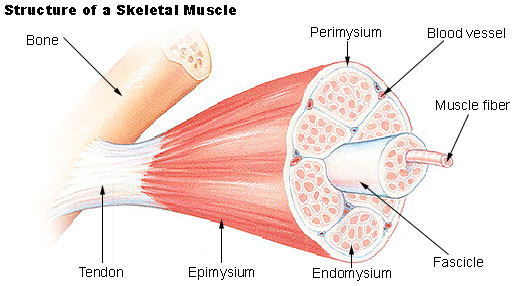
\includegraphics[height=4cm]{figures/epymisium.jpg}
    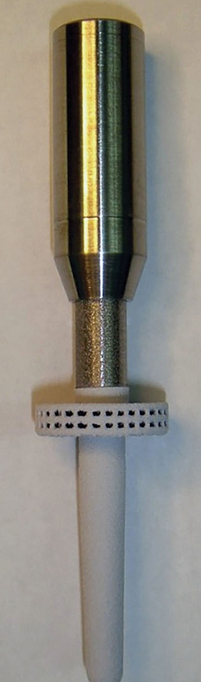
\includegraphics[height=5cm]{figures/round-flange.png}
\end{frame}

\begin{frame}
    \frametitle{Experiment}

    \begin{itemize}
        \item Animals walk on treadmill at 2 km/h
        \item Record EMG approx. weekly for 14 weeks
        \item Compare to skin surface EMG at 19 weeks.
        \item Use signal-to-noise ratio to approximate signal quality
    \end{itemize}
    TMR
    \begin{itemize}
        \item Use force plates to assess weight bearing recovery.
    \end{itemize}
\end{frame}

\begin{frame}
    \frametitle{Results}
    
    \begin{itemize}
        \item Well-vascularised dermal integration into 90\% of flangeal pores
        \item Areas of poor integration led to downgrowth and debris to collect 
        \item Mean electrode impedance from \SI{1.3}{\kilo\ohm} to \SI{2.2}{\kilo\ohm} in-vivo
        \item TMR: Muscular atrophy, but regular weight bearing at 6 weeks.
    \end{itemize}

\end{frame}

\begin{frame}
    \frametitle{Results --- EMG}

    \begin{itemize}
        \item Higher SNR, but not statistically different \begin{itemize}
            \item Epymisium: 19.6 $\pm$ 7.4 dB
            \item Skin Surface: 6.65 $\pm$  7.63 dB 
        \end{itemize}
    \end{itemize}
    \begin{figure}[h]
    \centering
        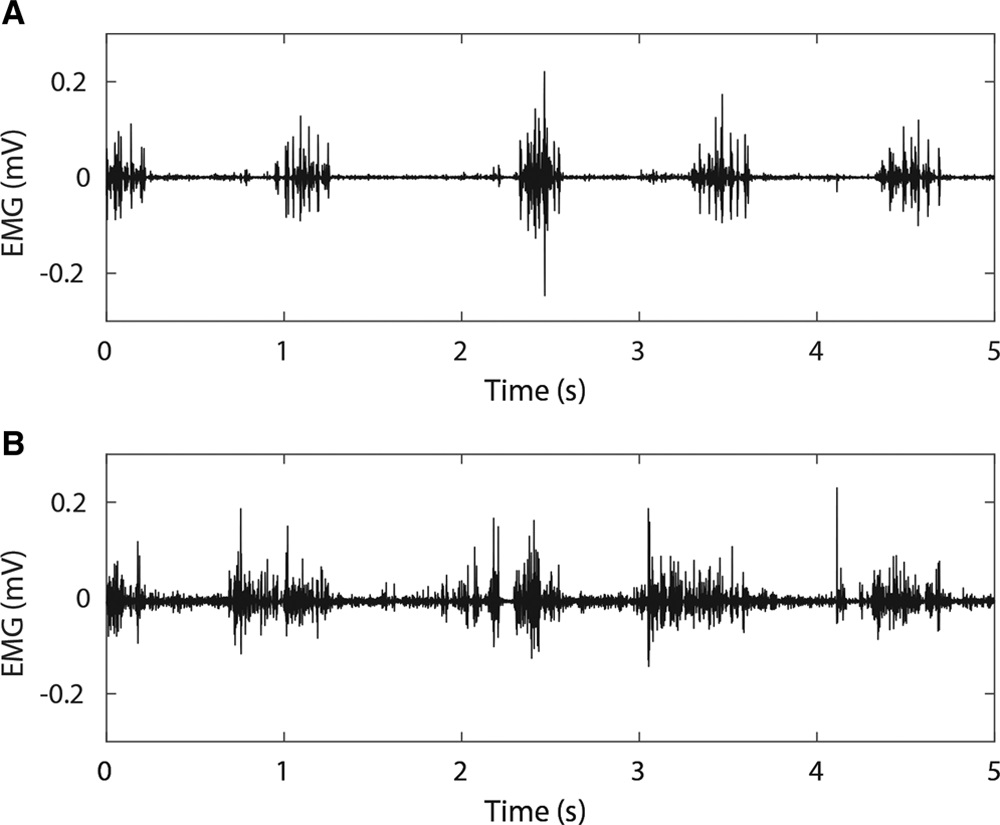
\includegraphics[width=0.5\textwidth]{figures/emg.jpeg}
    \caption{Traces at 19 weeks from same animal (A) Epymisial; (B) Skin surface}
    \label{fig:emg.jpeg}
    \end{figure}
\end{frame}